\documentclass[14pt,a4paper,oneside]{extarticle} % 

%% подключаем стандарт библиографии
\bibliographystyle{gost71u}

%% для "Abstract" в классе book
% \newenvironment{abstract}{}{}
% \usepackage{abstract}

%% подключаем преамбулу: в ней содержится подключение всех необходимых пакетов


% Русская локализация и кодировки
\usepackage{cmap}                % улучшенный поиск в PDF
\usepackage[T2A]{fontenc}        % кодировка шрифтов
\usepackage[utf8]{inputenc}      % кодировка исходного текста
\usepackage[russian]{babel}      % локализация и переносы

% Геометрия страницы: урезанные поля для максимальной печатной области
\usepackage[left=3cm,right=1.5cm,top=2cm,bottom=2cm,bindingoffset=0cm]{geometry}

% Интервалы и отступы
\usepackage{setspace}
\onehalfspacing                 % межстрочный интервал 1.5
\setlength{\parindent}{1.25cm}    % красная строка
\setlength{\parskip}{0pt}      % без дополнительного отступа между абзацами


% Работа с математикой
\usepackage{amsmath,amsfonts,amssymb,amsthm,mathtools}
\usepackage{icomma}

% Шрифты для математики
\usepackage{euscript}           % шрифт "Евклид"
\usepackage{mathrsfs}           % красивый мат. шрифт

% Русские списки
\usepackage{enumitem}
\makeatletter
\AddEnumerateCounter{\asbuk}{\russian@alph}{щ}
\makeatother

% Работа с картинками и таблицами
\usepackage{graphicx,caption,wrapfig,float}
\captionsetup{justification=centering, font=small}
\graphicspath{{images/}{images2/}}     % папки с картинками
\setlength{\fboxsep}{3pt}
\setlength{\fboxrule}{1pt}
\usepackage{array,tabularx,tabulary,booktabs,longtable,multirow}

% Код и листинги
\usepackage{listings}
\lstset{basicstyle=\small\ttfamily, columns=flexible, breaklines=true}

% TikZ
\usepackage{tikz}
\usetikzlibrary{graphs,graphs.standard}

% Гиперссылки
\usepackage[unicode, pdftex, hidelinks]{hyperref}

% Отступ перед первым абзацем в каждом разделе
\usepackage{indentfirst}

%% Верхний колонтитул
%\usepackage{fancyhdr}
%\pagestyle{fancy}


\begin{document}
    %% титульник
    \begin{center}
    %% *название института*
    \large\textbf{Министерство образования и науки Российской Федерации \\
    Московский физико-технический институт (государственный
    университет)} \\
    \vspace{1cm}

    %% *факультет/физтех-школа*
    Физтех-школа аэрокосмических технологий \\

    %% *название базовой кафедры и лаборатории*
    %% в случае ненадобности можно удалить
    Кафедра вычислительной физики \\

    \vspace{3em}

    Выпускная квалификационная работа бакалавра
\end{center}

\begin{center}
    \vspace{\fill}
    %% *название вашей работы*
    \LARGE{Расчетно-экспериментальное исследование применения аберраторов для акустической левитации}

    \vspace{\fill}
\end{center}


\begin{flushright}
    \textbf{Автор:} \\
    Студент группы Б03-101\\
    Куланов Александр Владимирович \\
    \vspace{2em}
    \textbf{Научный руководитель:} \\
    к.ф.-м.н.\\
    Беклемышева Катерина Алексеевна \\
    \vspace{2em}
\end{flushright}

\vspace{7em}

\begin{center}
    %% *лого*
    
\includegraphics[width=100 pt]{MIPT_logo.jpg}\\
    Москва \the\year{}
\end{center}

%% выключаем отображение номера для этой страницы (титульник)
\thispagestyle{empty}

\newpage
\setcounter{page}{2}
\fancyfoot[c]{\thepage}
%% *надпись над верхним колонтинулом*
%% в случае ненадобности можно удалить
%\fancyhead[L]{Расчетно-экспериментальное исследование применения аберраторов для акустической левитации}
%\fancyhead[R]{}
    %% аннотоция
    \begin{abstract}

    \begin{center}
        \large{Расчётно-экспериментальное исследование применения аберраторов для акустической левитации} \\
    \large\textit{Куланов Александр Владимирович} \\[1 cm]

    Основной целью данной работы является исследование акустической левитации в воде с помощью математического моделирования и физического эксперимента. Практический интерес представляет изучение применимости выбранного численного метода, а так же аберраторов как способа влияния на получаемое акустическое поле. Для численного эксперимента используется решатель на основе сеточно-характеристического метода.
    
    РЕЗУЛЬТАТЫ

    \end{center}

\end{abstract}
\newpage
    %% содержание
    \tableofcontents{}
    \newpage

    \section{Введение}
\label{sec:Chapter0} \index{Chapter0}
\subsection{Актуальность}
Акустическая левитация представляет собой бесконтактный метод удержания и манипуляции телами в жидкой или газообразной среде за счёт действия сил акустического давления, возникающих при взаимодействии акустических волн с объектом. За последние десятилетия эта технология приобрела широкое признание в различных областях науки и техники благодаря своей способности минимизировать механические и химические взаимодействия с удерживаемым образцом. Она находит применение в многих инженерных приложениях, например, в фармацевтической области \cite{appliance_medicine}, машиностроении \cite{appliance_bearings} и прецизионной робототехнике \cite{appliance_robot}. В частности, одним из приложений является необходимость бесконтактного позиционирования биологических тканей в задаче биопечати. 

Существуют различные технические способы управления акустическим полем. К примеру, использование отражателей сложной формы в совокупности с массивом излучателей исследовано в \cite{nature_acoustics}. Другим подходом оптимизации акустических левитаторов является использование акустических аберраторов — специальных элементов, способных искажать фазу или амплитуду акустических волн для формирования заданного пространственного распределения давления. Такие аберраторы позволяют целенаправленно управлять звуковым полем, создавать нужную форму потенциала и задавать положение левитируемых объектов, не прибегая к использованию сложных массивов излучателей.

\subsection{Цель работы}

Настоящая работа посвящена численному моделированию акустической левитации с учётом применения аберрирующих элементов. Исследуется влияние параметров аберраторов на структуру акустического поля, полученная картина потенциала Горького и реальная устойчивость положения левитируемых объектов. Результаты могут быть использованы при проектировании перспективных систем для микро- и макроманипуляции. Для достижения поставленной цели были поставлены следующие задачи:
\begin{enumerate}
	\item Разработка и создание экспериментальной установки, позволяющей проводить физические эксперименты по акустический левитации в жидкости с возможностью использования различных излучателей
	\item Разработка или выбор готового программного комплекса, с помощью которого проводится моделирование физического эксперимента
\end{enumerate}

\newpage
 
    \section{Математическая модель}
\label{sec:Chapter1} \index{Chapter1}

\subsection{Система уравнений акустики}
Основой для описания исследуемой среды является модель линейной упругости. Тогда в общем случае, согласно \cite{kondaurov}

\begin{equation}
	\begin{aligned}
		\rho \dot{\vec{v}} & =\nabla \cdot \mathbb{T}+\vec{f} \\
		\dot{\mathbb{T}} & =\mathbf{q}: \dot{\varepsilon}+\mathbf{F}
	\end{aligned}
\end{equation}

Здесь $\rho$ - плотность в данной точке, $\vec{v}$ - скорость частиц в данной точке, $\mathbb{T}$ - тензор напряжений в данной точке, $\varepsilon$ - тензор деформаций в данной точке, $\vec{f}$ и $\mathbf{F}$ - силы, $\mathbf{q}$ - тензор упругих коэффициентов. Далее везде силы примем равными нулю, согласно постановке задачи. Пользуясь малостью смещения, используем выражения для тензора малых деформаций

\begin{equation}
	\varepsilon=\frac{1}{2}\left(\nabla \otimes \vec{r}+\vec{r} \otimes \nabla\right)
\end{equation}

Здесь $\vec{r}$ - вектор смещения в данной точке, $\otimes$ - оператор тензорного умножения. Дифференцируя это выражения по времени и подставляя в исходную систему, получаем

\begin{equation}
	\begin{aligned}
		\rho \dot{\vec{v}} & =\nabla \cdot \mathbb{T} \\
		\dot{\mathbb{T}} & =\frac{1}{2} \mathbf{q}:\left(\nabla \otimes \vec{v}+ \vec{v} \otimes \nabla \right)
	\end{aligned}
\end{equation}

Воспользуемся теперь тем, что исследуемая среда изотропна, то есть свойства одинаковы для любого направления в пространстве. Известно, что для такого материала количество независимых коэффициентов в тензоре $\mathbf{q}$ равно двум. Их называют параметры Ламе и обычно обозначают $\lambda$, $\mu$. Полезно также представить их выражения через модуль Юнга $E$ и коэффициент Пуассона $\nu$

\begin{equation}
	\begin{aligned}
		\lambda & =\frac{E \nu}{(1+\nu)(1-2 \nu)} \\
		\mu & =\frac{E}{2(1+\nu)} .
	\end{aligned}
\end{equation}

Итого, для изотропного случая можно записать

\begin{equation}
	\label{eq:isotropic}
	\begin{aligned}
		\rho \dot{\vec{v}} & =\nabla \cdot \mathbb{T} \\
		\dot{\mathbb{T}} & =\lambda(\nabla \cdot \vec{v}) \mathbb{I}+\mu\left(\nabla \otimes \vec{v}+ \vec{v} \otimes \nabla\right)
	\end{aligned}
\end{equation}

Остается последний шаг преобразования. Применим акустическое приближение: тензор напряжений зависит только от одного скалярного параметра $p$, который называют давлением, и выражается через единичный тензор $\mathbb{I}$. Модуль сдвига $\mu$ считается равен нулю.

\begin{equation}
	\begin{aligned}
		\mathbb{T} = -p \mathbb{I}
	\end{aligned}
\end{equation}

Эта модель хорошо подходит для описания жидкостей, что и требуется в настоящей работе. Традиционно переобозначим $\lambda$ за $K$ --- модуль всестороннего сжатия. Наконец,  подставляя это выражение в \ref{eq:isotropic}, получаем

\begin{equation}
	\begin{aligned}
		\rho \dot{\vec{v}} & =-\nabla (p \mathbb{I}) \\
		\dot{p} & =-K(\nabla \cdot \vec{v})
	\end{aligned}
\end{equation}

\subsection{Выражения для коэффициентов прохождения и отражения волны}

Для некоторых дальнейших рассуждений полезно понимать, какая часть волны проходит через контактную границу, а какая отражается обратно. В \cite{kazakov} приведено более подробное рассуждение, в настоящей же работе ограничимся соотношениями для нормально падающей на контактную границу волны:

\begin{equation}
	\label{eq:refl}
	\begin{aligned}
		R=\frac{Z_2-Z_1}{Z_2+Z_1} \\ 
		T=\frac{2 Z_2}{Z_2+Z_1}
	\end{aligned}
\end{equation}

Здесь $R$ - коэффициент отражения по амплитуде, $T$ - коэффициент прохождения по амплитуде. Возводя их в квадрат можно получить коэффициенты по энергии, но они не понадобятся. Индексам  "1"\ и "2"\ соответствуют величины в среде из которой и в которую бежит волна соответственно. Также важное обозначение 
\begin{equation}
	Z = \sqrt{\frac{K}{\rho}} = \rho c
	\label{impedance}
\end{equation}
--- акустический импеданс среды, величина, характеризующая сопротивление среды распространению звуковых волн, $c$ --- скорость звука в среде.

\subsection{Потенциал Горькова}
Потенциал Горькова --- это скалярная функция, отрицательный градиент которой описывает силу, действующую на малую частицу сферической формы в акустическом поле. Оригинальную формулу можно найти в \cite{gorkov}, а в настоящей работе будем использовать безразмерный потенциал, удобный для реализации в программном коде:

\begin{equation}
	U = \frac{\sqrt{ \langle p'^2 \rangle }}{3} - \frac{\sqrt{ \langle v'^2 \rangle }}{2}
\end{equation}

\begin{equation}
	\langle p'^2 \rangle = \langle p^2 \rangle - \langle p \rangle^2, \quad
	\langle v'^2 \rangle = \langle \mathbf{v}^2 \rangle - \langle \mathbf{v} \rangle^2
\end{equation}
Здесь давление и скорость приведены к безразмерной форме делением на $\rho c$ и $c$ соответственно.

\newpage

    \section{Описание численного метода}
\label{sec:Chapter2} \index{Chapter2}

\subsection{Сеточно-характеристический метод}
В настоящей работе используется сеточно-характеристический численный метод (СХМ). В самой общей постановке и подробно этот метод описан в \cite{kholodov}, а для системы уравнений акустики подробно рассмотрен, помимо прочего, в \cite{kazakov}. Для настоящей работы приведем краткое описание построения и применения данного метода. 

Для произвольной трехмерной области рассматривается гиперболическая система уравнений: 

\begin{equation}
	\frac{\partial \vec{u}}{\partial t}+\sum_{i=1}^3 \mathbf{A}_i \frac{\partial \vec{u}}{\partial x_i}=0 .
\end{equation}

Здесь матрицы $\mathbf{A}_i$ не зависят от пространственных координат и времени. Тот факт, что система гиперболическая, то есть её матрицы имеют полный набор собственных векторов и только вещественные собственные числа, позволяет разбивать эту систему на независимые уравнения переноса. Для этого необходимо представить исходную матрицу в виде спектрального разложения

\begin{equation}
	\mathbf{A}=\mathbf{U}^{-1} \boldsymbol{\Lambda} \mathbf{U}
\end{equation}
где $\mathbf{U}^{-1}$, $\mathbf{U}$ --- матрицы собственных векторов и строк соответственно. Далее, переходя к инвариантам Римана $\vec{r} = \mathbf{U} \vec{u}$, получаем

\begin{equation}
	\frac{\partial \vec{r}}{\partial t}+\boldsymbol{\Lambda} \frac{\partial \vec{r}}{\partial x}=0
\end{equation}
Так как матрица $\boldsymbol{\Lambda}$ диагональна, система распадается на независимые скалярные уравнения переноса. Для полученных одномерных уравнений применяется главная идея сеточно-характеристического метода. Из точки на временном слое $n+1$ выпускается характеристика, вдоль которой сохраняется значение решения. Далее функция интерполируется в точке пересечения этой характеристики с предыдущим временным слоем. После этого производится обратное преобразование $\vec{u} = \mathbf{U}^{-1} \vec{r}$. Сказанное выше проиллюстрировано на рисунке \ref{fig:gcm}:

\begin{figure}[H]
	\centering
	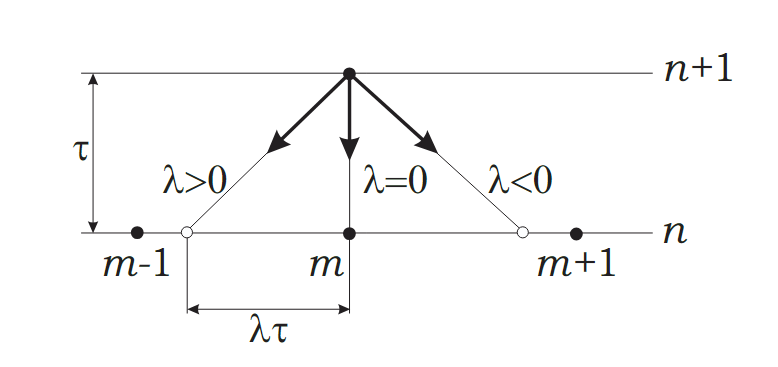
\includegraphics[width=0.7\textwidth]{gcm.png}
	\caption{Иллюстрация сеточно-характеристического метода в одномерном случае}
	\label{fig:gcm}
\end{figure}

Для системы уравнений акустики спектральное разложение выглядит довольно просто и было описано в \cite{kazakov}. Приведем лишь результат разложения. Вдоль направления $\vec{e}$ оно выглядит следующим образом:

\begin{equation}
	\mathbf{A} = \frac{1}{2}
	\begin{pmatrix}
		\vec{e} & \vec{e} & \vec{e'} & \vec{e''} \\
		c\rho & -c\rho & 0 & 0
	\end{pmatrix}
	\begin{pmatrix}
		c & 0 & 0 & 0 \\
		0 & -c & 0 & 0 \\
		0 & 0 & 0 & 0 \\
		0 & 0 & 0 & 0
	\end{pmatrix}
	\begin{pmatrix}
		\vec{e}^T & \dfrac{1}{c\rho} \\
		\vec{e}^T & -\dfrac{1}{c\rho} \\
		2\vec{e'}^T & 0 \\
		2\vec{e''}^T & 0
	\end{pmatrix}
\end{equation}
В данном контексте $\vec{e}$, $\vec{e'}$, $\vec{e''}$ образуют правую тройку, а собственные значения $c$ матрицы $\mathbf{A}$ равны

\begin{equation}
	\begin{aligned}
		c &= \pm \sqrt{\frac{K}{\rho}}, \\
		c &= 0
	\end{aligned}
\end{equation}

\subsection{Программный комплекс}
В настоящей работе используется программный комплекс, реализующий СХМ в 3D на языке Python. Его автором является А. В. Васюков \cite{gcm}. Выбор именно такого комплекса заключается в простоте использования и удобстве доработки, однако пришлось жертвовать скоростью расчетов. Расчеты производятся на ортогональной сетке, примерное время одного расчета --- десятки минут. Простота использования заключается в удобстве понимания и написания программного кода на языке Python, благодаря чему без особых усилий можно варьировать граничные условия и параметры среды. Проще говоря, при таком подходе большее количество сил и времени можно потратить на создание экспериментальной установки, что в настоящей работе оказалось нетривиальной задачей. Визуализация и контроль решения производились в среде ParaView, а так же средствами библиотеки matplotlib.

\newpage

    \section{Постановка задачи и эксперимента}
\label{sec:Chapter3} \index{Chapter3}

\subsection{Постановка задачи}
Как было сказано ранее, основной целью работы является изучение применения аберраторов для акустической левитации в воде. Исходя из этого были сформулированы требования к экспериментальной установке:
\begin{itemize}
	\item Главным инструментом для контроля формы распределения акустического давления является аберратор, то есть не используются матрицы из излучателей (используется один излучатель), а так же отражатели в форме, отличной от плоской.
	\item В качестве излучателя используется пьезоэлемент. В данном случае это решение безальтернативное.
	\item Диапазон доступных частот в 10--100 кГц и величина скорости звука в воде накладывают ограничения на размер резервуара для воды.
\end{itemize}
В качестве формы аберратора был выбран достаточно простой синусоидальный профиль, чтобы его можно было изготовить не прибегая к сложным технологиям. 
\subsection{Пьезоэлектрический эффект}
Как было сказано ранее, в экспериментальной установке излучателем является пьезоэлемент, так что следует привести краткие сведения о том, что это такое. Пьезоэлектрический эффект представляет собой физическое явление, заключающееся в возникновении электрического заряда на поверхности некоторых кристаллических материалов при их механическом деформировании. Этот эффект наблюдается в веществах с анизотропной кристаллической структурой, не обладающей центром симметрии. Он проявляется в двух формах: прямой и обратной.

Прямой пьезоэлектрический эффект заключается в генерации электрического потенциала в ответ на приложенное механическое воздействие (сжатие, растяжение, изгиб и др.). Это происходит вследствие изменения положения ионов в кристаллической решётке, что приводит к поляризации материала и возникновению поверхностного заряда. Сила возникшего электрического поля пропорциональна величине механической деформации. Обратный пьезоэлектрический эффект представляет собой деформацию кристалла под действием внешнего электрического поля. Это связано с перераспределением внутренних сил в кристаллической решётке, вызывающим изменение её геометрических размеров.

Наиболее ярко выраженные пьезоэлектрические свойства наблюдаются у таких материалов, как кварц, турмалин, титанат бария, цирконат-титанат свинца (PZT, пьезоэлементы из него используются в настоящей работе), а также у некоторых полимеров, например поливинилиденфторида (PVDF).

Благодаря способности преобразовывать электрический сигнал в механический такой же формы, пьезоэлемент отлично подходит для генерации синусоидальных волн, которые необходимы для акустической левитации.
\subsection{Создание экспериментальной установки}

\newpage
 
    \section{Результаты}
\label{sec:Chapter4} \index{Chapter4}

\subsection{Результаты численных расчетов}
Ниже представлены результаты моделирования для постановки с кольцевым источником с частотой 38 кГц. На рисунке \ref{fig:source} представлен типичный вид кольцевого излучателя на расчетной сетке.
\begin{figure}[H]
	\centering
	\includegraphics[width=0.8\textwidth]{source_bottom.png}
	\caption{Кольцевой излучатель, вид снизу на расчетную область}
	\label{fig:source}
\end{figure}

На рисунках \ref{fig:cos005}, \ref{fig:cos01}, \ref{fig:cos02}, \ref{fig:cos02} отображены результаты моделирования аберратора в виде полупериода синуса. Как можно видеть, при малой высоте профиля форма потенциала почти не отличается от равномерной, как на рис. \ref{fig:uniform}. При увеличении высоты в некоторый момент по бокам от вершины возникают две отдельные области минимума потенциала, вместо одной протяженной. 

\begin{figure}[H]
	\centering
	\includegraphics[width=0.8\textwidth]{cos005.png}
	\caption{Результат расчета для кольцевого пьезоэлемента 38 кГц, аберратор синусоидальной формы}
	\label{fig:cos005}
\end{figure}

\begin{figure}[H]
	\centering
	\includegraphics[width=0.8\textwidth]{cos01.png}
	\caption{Результат расчета для кольцевого пьезоэлемента 38 кГц, аберратор синусоидальной формы}
	\label{fig:cos01}
\end{figure} 

\begin{figure}[H]
	\centering
	\includegraphics[width=0.8\textwidth]{cos02.png}
	\caption{Результат расчета для кольцевого пьезоэлемента 38 кГц, аберратор синусоидальной формы}
	\label{fig:cos02}
\end{figure} 

\begin{figure}[H]
	\centering
	\includegraphics[width=0.8\textwidth]{cos03.png}
	\caption{Результат расчета для кольцевого пьезоэлемента 38 кГц, аберратор синусоидальной формы}
	\label{fig:cos03}
\end{figure}

\begin{figure}[H]
	\centering
	\includegraphics[width=0.8\textwidth]{uniform.png}
	\caption{Результат расчета для кольцевого пьезоэлемента 38 кГц без аберратора}
	\label{fig:uniform}
\end{figure}

Ниже на рисунках \ref{fig:par005}, \ref{fig:par001}, \ref{fig:par0005} приведены результаты моделирования параболического аберратора. Его ширина соответствует диаметру излучателя. Смотря на результаты, можно сделать вывод, что параболических аберратор сам по себе не сильно меняет картину потенциала.

\begin{figure}[H]
	\centering
	\includegraphics[width=0.8\textwidth]{par005.png}
	\caption{Результат расчета для кольцевого пьезоэлемента 38 кГц, аберратор параболической формы}
	\label{fig:par005}
\end{figure} 

\begin{figure}[H]
	\centering
	\includegraphics[width=0.8\textwidth]{par001.png}
	\caption{Результат расчета для кольцевого пьезоэлемента 38 кГц, аберратор параболической формы}
	\label{fig:par001}
\end{figure} 

\begin{figure}[H]
	\centering
	\includegraphics[width=0.8\textwidth]{par0005.png}
	\caption{Результат расчета для кольцевого пьезоэлемента 38 кГц, аберратор параболической формы}
	\label{fig:par0005}
\end{figure}

Наконец, для цилиндрического пьезоэлемента на 108 кГц рассмотрен аберратор в виде синусоидального профиля. Результаты представлены на рисунках \ref{fig:sin1}, \ref{fig:sin2}, \ref{fig:sin3}, \ref{fig:sin4}. Как видно из рисунков, количество периодов слабо влияет на получаемую картину потенциала. Интересным кажется случай на рис. \ref{fig:sin2} --- в некоторых областях форма потенциала похожа на обратную форму аберратора.

\begin{figure}[H]
	\centering
	\includegraphics[width=0.8\textwidth]{sin1.png}
	\caption{Результат расчета для цилиндрического пьезоэлемента 108 кГц, аберратор синусоидальной формы}
	\label{fig:sin1}
\end{figure} 

\begin{figure}[H]
	\centering
	\includegraphics[width=0.8\textwidth]{sin2.png}
	\caption{Результат расчета для цилиндрического пьезоэлемента 108 кГц, аберратор синусоидальной формы}
	\label{fig:sin2}
\end{figure} 

\begin{figure}[H]
	\centering
	\includegraphics[width=0.8\textwidth]{sin3.png}
	\caption{Результат расчета для цилиндрического пьезоэлемента 108 кГц, аберратор синусоидальной формы}
	\label{fig:sin3}
\end{figure}

\begin{figure}[H]
	\centering
	\includegraphics[width=0.8\textwidth]{sin4.png}
	\caption{Результат расчета для цилиндрического пьезоэлемента 108 кГц, аберратор синусоидальной формы}
	\label{fig:sin4}
\end{figure}

\subsection{Результаты физического эксперимента}
К сожалению, автору не удалось получить устойчивую картину акустической левитации. Ни один из трех используемых пьезоэлементов не создал достаточно мощное поле. Наглядным показателем является рябь на воде при включении, однако она не наблюдалась. Это может быть связано с различными факторами. Например, неточно сконструированный согласующий слой, а именно наличие пузырьков в толще эпоксидной смолы или погрешность толщины. Однако наиболее вероятной причиной является недостаточная мощность усилителя. Об этом свидетельствует тот факт, что при работе он быстро (около 30 секунд) перегревается, ток после старта начинает падать, а синусоидальный сигнал искажается. При этом в слышимом диапазоне все три излучателя издавали достаточно громкий звук при работе, но, судя по всему, это не является показателем.

Самый близкий к удачному результат был получен с кольцевым пьезоэлементом на частоте 60 кГц при работе в сильно соленой воде. Была предпринята попытка довести плотность воды почти до плотности PLA-пластика, чтобы частички обладали почти нейтральной плавучестью. При опускании с поверхности, на несколько секунд наблюдалась практически полная остановка одной из частиц на некотором расстоянии над излучателем, но вскоре после этого частица утонула. На рисунке \ref{fig:final} можно наблюдать этот момент. Соленая вода была мутной, поэтому качество фотографии оставляет желать лучшего.

\begin{figure}[H]
	\centering
	\includegraphics[width=1\textwidth]{final.jpg}
	\caption{Момент замедления частицы над излучателем}
	\label{fig:final}
\end{figure} 

В связи с тем, что не удалось получить устойчивую картину в простейшем случае, физических экспериментов с аберратором проведено не было. 
\newpage
 
    \section{Заключение}
\label{sec:Chapter5} \index{Chapter5}
Подводя итоги, перечислим основные результаты работы:
\begin{enumerate}
	\item В ходе численного моделирования были получены различные картины потенциала Горькова для разных форм аберратора: полупериод косинуса, парабола, периоды синуса. В общем, можно сказать, что управление акустическим полем с помощью аберраторов возможно, но с отражателем плоской формы не очень эффективно.
	\item Хотя физический эксперимент провести не удалось, получены ценные знания и опыт по созданию установки для акустической левитации. Было выявлено, что схема на основе усилителя мощностью 25 Вт для звуковой аппаратуры не достаточно для получения устойчивой картины стоячих волн в воде в условиях, рассмотренных в работе. Для хорошего усиления сигнала для пьезоэлемента нужны специализированные усилители для ультразвуковых частот. Помимо этого автором получен опыт пайки пьезоэлементов, печати форм и заливки их эпоксидной смолой. Было подтверждено, что эпоксидная смола хорошо подходит для электроизоляции и герметизации от воды. 
\end{enumerate}
\newpage
 


    %% НЕ ТРОГАЙТЕ!!!
    \nocite{*}
    % \cleardoublepage
    % \markboth{}{}  % <-- Это вручную задаёт метки
    \bibliography{references}

    %% в зависимости от надобности подключаем раздел "Приложение"
    % \newpage
    % \section*{Приложение}
\addcontentsline{toc}{section}{Приложение}
\label{sec:Apendix} \index{Apendix}

Здесь необходимо написать приложение, которое вы должны придумать самостоятельно.

\end{document}
